\documentclass[12pt]{article}
%\usepackage[latin1]{inputenc}
\usepackage[utf8x]{inputenc}
\usepackage[spanish,es-noshorthands]{babel}
\usepackage{amsmath}
\usepackage{amsthm}
\usepackage{graphicx}
\usepackage{wrapfig}
\usepackage{tabularx}
\usepackage{multicol}
\usepackage{standalone}
\usepackage{float}
\usepackage{anysize}
\usepackage{tikz}
\usetikzlibrary{patterns}
\usetikzlibrary{decorations.pathmorphing,patterns}
\usetikzlibrary{arrows,calc,patterns,decorations.markings}
\usetikzlibrary{positioning}
\spanishdecimal{.}
\linespread{1.3}
\numberwithin{equation}{section}
\marginsize{1.5cm}{1.5cm}{0cm}{2cm}
\author{M. en C. Gustavo Contreras Mayén.}
\title{Métodos numéricos para matrices - Tarea \\ \begin{Large}Curso de Fí­sica Computacional\end{Large}}
\date{ }
\begin{document}
\fontsize{14}{14}\selectfont
\maketitle
\begin{enumerate}
\item El sistema mostrado en la figura consiste en $n$ resortes lineales que soportan $n$ masas. La constante de los resortes se indican por $k_{i}$, mientras que el peso de las masas, es $W_{i}$ y $x_{i}$ son los desplazamientos de las masas (medidos de la posición donde el resorte no está deformado). La llamada \emph{formulación de desplazamiento} se obtiene escribiendo la ecuación de equilibrio para cada masa y sustituyendo $F_{i} = k_{i}(x_{i + 1} - x_{i})$ para la fuerza en los resortes. El resultado es un conjunto de ecuaciones simétricas y tridiagonal:
\\
\begin{minipage}{0.5\textwidth}
\[ \begin{split}
(k_{1} + k_{2}) \: x_{1} - k_{2} \: x_{2} =& \: W_{1} \\
-k_{i} \: x_{i-1} + (k_{i} + k_{i+1}) \: x_{i} - k_{i+1} \: x_{i+1} =& \:  W_{i}, \\
-k_{n} \:  x_{n-1} + k_{n} \: x_{n} =& \: W_{n}
\\
\\
 i = 2, 3, \ldots, n-1r
\end{split} \]
\end{minipage}
\begin{minipage}{0.5\textwidth}
\begin{figure}[H]
	\centering
	\includestandalone{Figuras/Sistema_Masas_Tarea}
\end{figure}
\end{minipage}
\\
\\
\\
Escribe un programa que resuelva este conjunto de ecuaciones para los valores dados de $n$, $k$ y $W$. Considera $n=5$ y 
\[ \begin{split} 
k_{1} = k_{2} = k_{3} = 10 \mbox{ N/mm} \hspace{2cm} k_{4} = k_{5} = 5 \mbox{ N/mm} \\
W_{1} = W_{3} = W_{5} = 100 \mbox{ N} \hspace{2cm} W_{2} = W_{4} = 50 \mbox{ N}
\end{split} \]
\item Sea $\textbf{A}$ una matriz tridiagonal de $50 \times 50$:
\[
\mathbf{A} = \begin{bmatrix}
5 & -1 & & & & \\
-1 & 5 & -1 & & &  \\
 & -1 & 5 & -1 & & \\
 & & \ddots & \ddots & \ddots & \\
 & & & -1 & 5 & -1 \\
 & & & & -1 & 5
\end{bmatrix}
\]
Considera el problema $\mathbf{A \: x = B}$ para $50$ vectores de la forma:
\begin{align*}
b_{1} &= [1, 2, \ldots, 48, 49, 50]^{T} \\
b_{2} &= [2, 3, \ldots, 49, 50, 1]^{T} \\
b_{3} &= [3, 4, \ldots, 50, 1, 2]^{T} \\
\ldots \\
\ldots \\
b_{50} &= [50, 1, \ldots, 47, 48, 49]^{T} \\
\end{align*}
Resuelve el problema para cada vector $\mathbf{b_{i}}$.
\item Calcula las corrientes $i_{1}$ a $i_{4}$ del siguiente circuito:
\begin{figure}[H]
	\centering
	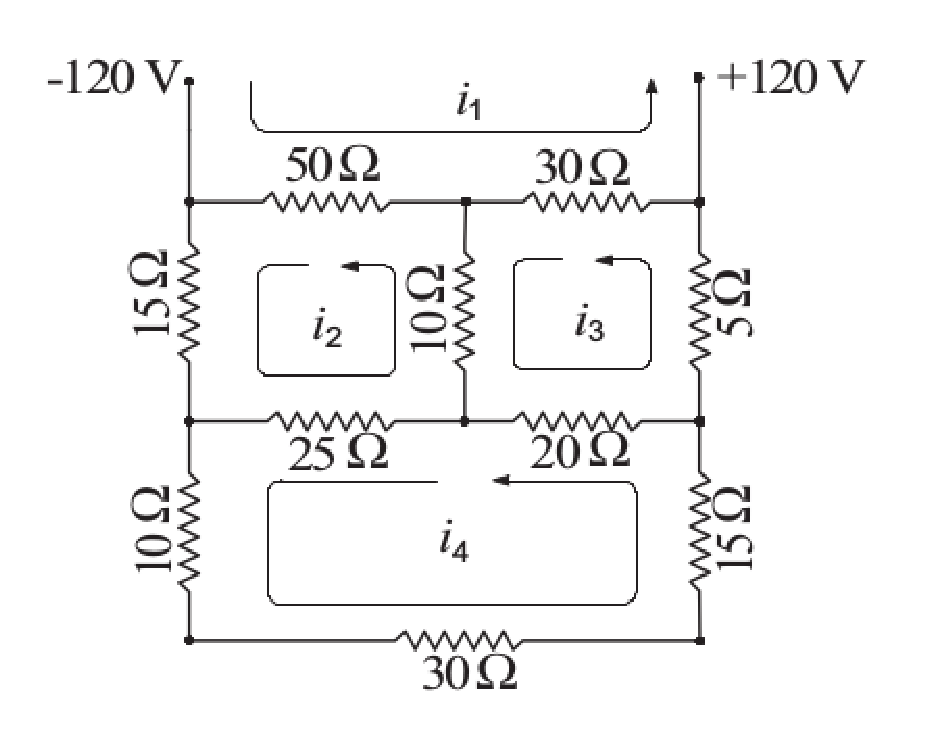
\includegraphics[scale=0.7]{Imagenes/Circuito_Tarea_2018_2.eps}
\end{figure}
\end{enumerate}	
\end{document}